\documentclass[a4paper]{report} % set paper size

\usepackage[utf8]{inputenc}
\usepackage {url}
\usepackage[top=2.54cm, bottom=2.54cm, left=2.54cm, right=2.54cm]{geometry} % set margin
\usepackage{amsfonts} % for set names
\usepackage{amsmath} % for equation system
\usepackage{amsthm} % for theorem block
\usepackage{fixltx2e} % for subscript
\usepackage{fancyhdr} % for footer/headline modification
\usepackage{xcolor}
\usepackage{graphicx} % for image insertion
\usepackage[ruled,vlined]{algorithm2e} % for algorithm integration

\pagestyle{fancyplain} % for footing modification on all pages
%\fancyhf{}
\renewcommand{\headrulewidth}{0pt} % remove decorative lign
\fancyhead[L]{Alexandre Devienne BA1 EL 2014}

\begin{document}

\section*{Autumn programming project : Recolor}
The program's organisation is as follows :
\begin{enumerate}
\item Read the inputs

The entire input is divided into 5 functions which read each section separetly (i.e.: all recoloring color together).
In alternance to the call of these functions, the tables and matrixes in which to store the data are dynamicly allocated in main using custom functions.

\item Process the inputs
    \begin{enumerate}
    \item Normalize and compare to the thresholds each pixels while reading them 
    \item Filtrage algorithm 
    \end{enumerate}
\item Print the output (a single function does this job)
\end{enumerate}

To furthermore show the abstraction made using function in this program we can consider the very basic functions : set\_border, copy\_2D\_tab and reset\_voisin.
Even though they are only called once in the program they 


re-utilisation :
dichotomie like search for seuillage
dynamic memory allocation for matrix and tables (even checks if the allocation is sucesful)

show abstraction/re-usage of fct
One particular thing to note is that my seuillage function is based on dicotomie search

analyse complexity of filtrage
set border : 2 + 2nbC + 2 nbL
1 + nbF * (nbL * nbC * (6+1 + 9 * 9+ 2) + nbC*nbL)
tot = nbF*nbC*nbL (90)


\begin{algorithm}
    \KwData{$image$ seuilée, $nbF$ number of filtrage}
    \KwResult{Image filtrée}
    \BlankLine
    Let $temp$ be a matrix of colors and size the original image\;
    Let $pixel$, $neighboor$ and $val$ be colors\;
    Let $T$ be a dictionnary as described in function below and of size $3$\;

    \BlankLine
    Set the border of $temp$ to black\;
    \For{$i \leftarrow 1$ \KwTo $nbF$}{
        \For{each $pixel$ in $image$ (border excepted)}{
            $val \leftarrow $ UNASSIGNED\;
            reset $T$ (remove all entry and set all integers to 0)\;
            \For{each $neighboor$ of $pixel$} {
                \If{$val = $ UNASSIGNED} {
                    $val \leftarrow $ \emph{insertInDictionnary}($neighboor$, $T$)\; 
                }
            }
            \If{$val = $ UNASSIGNED} {
                $val \leftarrow$ black \;
            }
            Set corresponding $pixel$ of $temp$ to $val$\; 
        }
        $image \leftarrow temp$\;
    }

\BlankLine
\SetKwProg{Fn}{Function}{}{}
\Fn{insertInDictionnary($color$, $T$)}
{
\KwIn{$color$ to insert in dictionnary $T$ of limited size, and which can contain a integer for each entry (colors)}
\KwOut{Color of resulting cell, or UNASSIGNED if cannot decide yet}
\BlankLine
\uIf{$color$ already in $T$} {
    increment corresponding integer by 1\;
    \If{$integer > 6$} {
        \KwRet $color$
    }
}
\uElseIf{$T$ full} {
    \KwRet black\;
}
\Else
{
    Store $color$ in new entry of $T$\;
    Set correponding integer to 1\;
}
\KwRet UNASSIGNED
}
\caption{Filtrage algorithm}
\end{algorithm}

\begin{figure}
\begin{center}
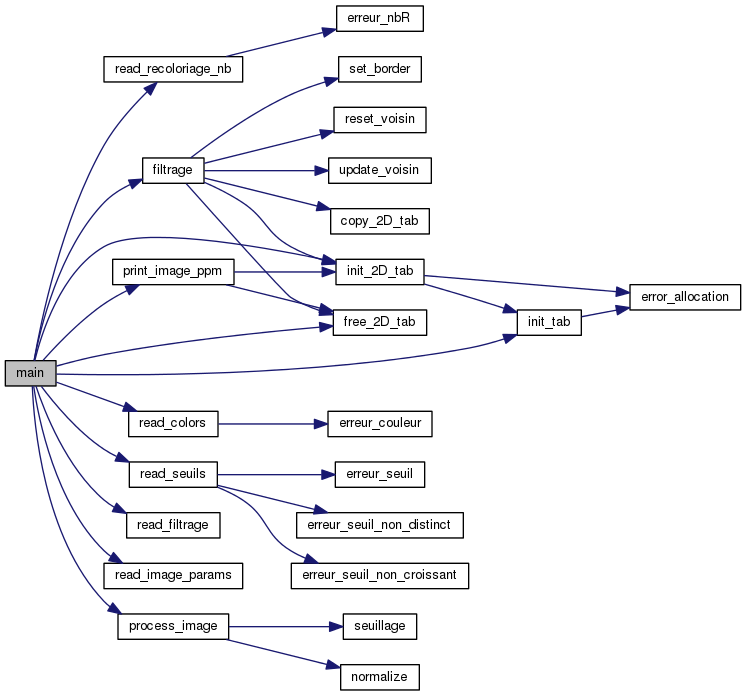
\includegraphics[scale=0.6]{graph.png}
\end{center}
\caption{Call graph}
\end{figure}

\end{document}
